\documentclass[12pt]{article}

\usepackage{sbc-template}

\usepackage{graphicx,url}

%\usepackage[brazil]{babel}   
\usepackage[latin1]{inputenc}  

\usepackage{amsmath}
\usepackage{amssymb} 
\usepackage{mathtools}

\usepackage{algorithm}
\usepackage[noend]{algpseudocode}

 
\newcommand{\Cfield}{\mathbb{C}}
\newcommand{\Rfield}{\mathbb{R}}

\newcommand{\norm}[1]{\left\lVert#1\right\rVert}

\sloppy

\title{Optimizing a Boundary Elements Method for Stationary
Elastodynamic Problems implementation with GPUs}

\author{Giuliano A. F. Belinassi\inst{1}, Rodrigo Siqueira\inst{1}, Ronaldo Carrion\inst{2}
, Alfredo Goldman\inst{1}, \\ Marco D. Gubitoso\inst{1} }


\address{Instituto de Matem�tica e Estat�stica (IME) -- Universidade de S�o Paulo
  (USP)\\
  Rua do Mat�o, 1010 -- S�o Paulo -- SP -- Brazil
\nextinstitute
  Escola Polit�cnica (EP)  -- Universidade de S�o Paulo (USP)\\
  Avenida Professor Mello Moraes, 2603 -- S�o Paulo -- SP -- Brazil
}

\begin{document} 

\maketitle

\begin{abstract}

The Boundary Element Method requires a geometry discretization to execute simulations, 
and it can be used to analyze the 3D stationary behavior of wave propagation in the soil. 
Such discretization involves generating two high computational power demanding matrices, 
and this article demonstrates how Graphical Processing Units (GPU) were used to accelerate 
this process. For an experiment with 4000 Mesh elements and 1600 Boundary elements, 
a speedup of 106.95 is obtained with such devices.

\end{abstract}
     
\section{Introduction}

Differential equations governing problems of Mathematical Physics only have analytical 
solutions in cases in which both the domain geometry, boundary and initial conditions 
are reasonably simple. Problems with arbitrary domains and fairly general boundary conditions 
can only be solved in an approximate way, for example, by numerical techniques. These techniques 
have experienced strong development due to the presence of increasingly powerful digital electronic 
computers, allowing the solution of complex mathematical problems. 

The Boundary Element Method (BEM) is a very efficient alternative for modeling unlimited 
domains, since it naturally satisfies the 
Sommerfeld radiation condition, also known as geometric damping.
Such method can be used to numerically model the 3D stationary behavior of wave propagation in the soil 
based on BEM with the objective of creating a computational tool which can assist in analysis such as 
evaluation of vibrations in the soil rising from machine tools operation or railway lines as well as 
to understand the role of soil during earthquakes or even in the design of offshore oil platforms.

With the invention of GPUs, several mathematical and engineering simulation problems were redesigned
to be implemented into GPUs to explore its massively parallel capabilities. However, 
first GPUs were designed to render graphics in real time, as a consequence, all the available 
libraries were graphical oriented such as OpenGL. These redesigns involved converting 
the original problem into a graphical domain, requiring deep knowledge of the selected 
graphical library. 

NVIDIA noticed a new demand for their products and created an API called CUDA to enable 
the use of GPUs in general purpose situation. CUDA has the concept of kernels, which are
 functions called from host to be executed in 
the GPU threads. Kernels are organized into a set of blocks wherein each block is a set 
of threads that cooperate with each other \cite{patterson:2007}.

GPU's memory is divided into global memory, local memory, and shared memory. First, it is 
a memory that all threads can access. Second, it is a memory that is private to a thread. 
Third, it is a  low-latency memory that is shared between all threads in the same block
\cite{patterson:2007}. CUDA provides a mechanism to access all of them.

Before discussing any parallelization technique or results, Section 2 presents a very brief mathematical 
formulation of BEM for Stationary Elastodynamic Problems and the meaning of some functions presented in 
the current work. Section 3 shows how the most computational expensive routine was optimized using GPUs. 
Section 4 discusses how the results were obtained. Section 5 presents and discusses the results. Finally, 
Section 6 provides an overview of our future work.

\section{Boundary Elements Method Background}


Without addressing details on the BEM formulation, the Boundary Integral Equation for Stationary
Elastodynamic Problems can be written as:

\begin{equation}
	c_{ij}u_{j}(\xi,\omega) + \int_S t_{ij}^*(\xi, x, \omega)u_j (x, \omega)\text{d}S(x) = \int_S u_{ij}^*(\xi, x, \omega) t_j(x, \omega)\text{d}S(x)
\end{equation}

After performing the geometry discretization, Equation (1) can still be represented in matrix form as:

\begin{equation}
	[H]\{u\} = [G]\{t\}
\end{equation}


Functions $u_{ij}^{*}(\xi, x, \omega)$ and $t_{ij}^{*}(\xi, x, \omega)$ (called fundamental solutions)
present a singular behavior when $\xi = x$ ordely $O(1/r)$, called weak singularity, and $O(1/r^2)$,
called strong singularity, respectively. The $r$ value represents the distance between $x$ and $\xi$
points.
To overcome this problem in the strong singularity, one use the artifice known as Regularization of 
the Singular Integral that can be expressed as follows:
%
\begin{equation}
\begin{split}
	c_{ij}(\xi)u_{j}(\xi, \omega) + \int_{S}\left[t_{ij}^{*}(\xi, x, \omega)_{\text{DYN}} - t_{ij}^{*}(\xi, x)_{\text{STA}} \right]u_{j}(x, \omega) \text{d}S(x) + \\
	+ \int_S t_{ij}(\xi, x)_\text{STA} u_j(x)\text{d}S(x) = \int_S u_{ij}^{*}(\xi, x, \omega)_{\text{DYN}} t_j(x, \omega)\text{d}S(x)	
\end{split}
\end{equation}
Where DYN = Dynamic, EST = Static. The integral of the difference between the dynamic and static nuclei, 
first one in Equation (3), does not present singularity when executed concomitantly as expressed because 
they have the same order in the both problems.


Algorithmically, equation (1) is implemented into a routine named $\texttt{Nonsingd}$, computing the
integral using the Gaussian Quadrature without addressing problems related to singularity. 
To overcome singularity problems, there is a special routine called $\texttt{Sing\_de}$ that uses an 
artifice known as Regularization of the Singular Integral. By last, $\texttt{Ghmatecd}$ is a routine 
developed to create both $H$ and $G$ matrices described in equation (2).


\section{Parallelization Strategies}

A parallel implementation of BEM began by analyzing and modifying a sequential code 
provided by \cite{carrion:02}. Gprof \cite{binutils}, a profiling tool by GNU, showed that the most time-consuming 
routine was $\texttt{Nonsingd}$. Since most calls to $\texttt{Nonsingd}$ were from $\texttt{Ghmatecd}$, most of the parallelization effort 
was focused on that last routine.

\subsection{Ghmatecd Parallelization}

Algorithm 1 shows the pseudocode of $\texttt{Ghmatecd}$ subroutine. Let $n$ be the number of mesh elements and $m$ the number of 
boundary elements. $\texttt{Ghmatecd}$ builds matrices $H$ and $G$ by computing smaller $3\times3$ matrices returned 
by $\texttt{Nonsingd}$ and $\texttt{Singi\_de}$.
%
\begin{algorithm}[H]
\caption{Creates $H, G \in \Cfield^{(3m)\times(3n)}$}
\begin{algorithmic}[1]
	\Procedure{Ghmatecd}{}
		\For{$j := 1, n$} 
			\For{$i := 1, m$}
				\State{$ii := 3(i-1) + 1;     jj := 3(j-1) + 1$}
				\If{$i == j$}
					\State{$Gelement, Helement \leftarrow \text{Sing\_de}(i)$}\Comment{two $3\times3$ complex matrices}					
				\Else
					\State{$Gelement, Helement \leftarrow \text{Nonsingd}(i, j)$}	
				\EndIf
				\State{$G[ii:ii+2][jj:jj+2] \leftarrow Gelement$}
				\State{$H[ii:ii+2][jj:jj+2] \leftarrow Helement$}
			\EndFor
	 \EndFor
	\EndProcedure
\end{algorithmic}
\end{algorithm}
%
There is no interdependency between all iterations in lines 2-3 loops, thus, all iterations can be computed 
in parallel. Since typically high-end CPUs have 8 cores, even a small number of mesh elements generate enough 
workload to use all CPUs resources if this strategy alone is used. On the other hand, a GPU contain thousands 
of processors, hence even a considerable large amount of elements may not generate a workload in a way that 
it consumes all the devices resources. Since $\texttt{Nonsingd}$ is the cause of the high time cost of $\texttt{Ghmatecd}$, 
the main effort was to implement
an optimized version of $\texttt{Ghmatecd}$, called $\texttt{Ghmatecd\_Nonsingd}$, that only computes the $\texttt{Nonsingd}$
case in the GPU, and leave $\texttt{Sing\_de}$ to be computed in the CPU after the computation of $\texttt{Ghmatecd\_Nonsingd}$ 
is completed. The pseudocode in Algorithm 2 pictures a new strategy where $\texttt{Nonsingd}$ is also computed in parallel.
Let $g$ be the number of Gauss quadrature points.

\begin{algorithm}[H]
\caption{Creates $H, G \in \Cfield^{(3m)\times(3n)}$ }
\begin{algorithmic}[1]
	\Procedure{Ghmatecd\_nonsingd}{}
		\For{$j := 1, n$} 
			\For{$i := 1, m$}
				\State{$ii := 3(i-1) + 1;     jj := 3(j-1) + 1$}
				\State{Allocate \textit{Hbuffer} and \textit{Gbuffer}, buffer of matrices $3 \times 3$ of size $g^2$}
				\If{$i \neq j$}
					\For{$y := 1, g$}
						\For{$x := 1, g$}
							\State{$\textit{Hbuffer}(x, y) \leftarrow \text{GenerateMatrixH}(i, j, x, y)$}
							\State{$\textit{Gbuffer}(x, y) \leftarrow \text{GenerateMatrixG}(i, j, x, y)$}
						\EndFor
					\EndFor
				\EndIf
				\State{$Gelement \leftarrow \text{SumAllMatricesInBuffer}(\textit{Gbuffer})$} 
				\State{$Helement \leftarrow \text{SumAllMatricesInBuffer}(\textit{Hbuffer})$}
				\State{$G[ii:ii+2][jj:jj+2] \leftarrow Gelement$}
				\State{$H[ii:ii+2][jj:jj+2] \leftarrow Helement$}
			\EndFor
	 \EndFor
	\EndProcedure
	\Procedure{Ghmatecd\_Sing\_de}{}
		\For{$i := 1, m$}
			\State{$ii := 3(i-1) + 1$}
			\State{$Gelement, Helement \leftarrow \text{Sing\_de}(i)$}	
			\State{$G[ii:ii+2][ii:ii+2] \leftarrow Gelement$}
			\State{$H[ii:ii+2][ii:ii+2] \leftarrow Helement$}
	 \EndFor
	\EndProcedure
	\Procedure{Ghmatecd}{} 
		\State{$\text{Ghmatecd\_Nonsingd}()$}
		\State{$\text{Ghmatecd\_Sing\_de}()$}
	\EndProcedure
		
\end{algorithmic}
\end{algorithm}

%\begin{algorithm}
%\caption{Creates $H, G \in \Cfield^{(3m)\times(3n)}$ without Sing_de part}
%\begin{algorithmic}[1]
%	\Procedure{Ghmatecd\_nonsingd}{}
%		\For{$j := 1, n$} 
%			\For{$i := 1, m$}
%				\State{$ii := 3(i-1) + 1;     jj := 3(j-1) + 1$}
%				\State{Allocate \textit{Hbuffer} and \textit{Gbuffer}, buffer of matrices $3 \times 3$ of size $g^2$}
%				\If{$i \neq j$}
%					\For{$y := 1, g$}
%						\For{$x := 1, g$}
%							\State{$\textit{Hbuffer}(x, y) \leftarrow \text{GenerateMatrixH}(i, j, x, y)$}
%							\State{$\textit{Gbuffer}(x, y) \leftarrow \text{GenerateMatrixG}(i, j, x, y)$}
%						\EndFor
%					\EndFor
%					\State{$Gelement \leftarrow \text{SumAllMatricesInBuffer}(\textit{Gbuffer})$} 
%					\State{$Helement \leftarrow \text{SumAllMatricesInBuffer}(\textit{Hbuffer})$}
%					\State{$G[ii:ii+2][jj:jj+2] \leftarrow Gelement$}
%					\State{$H[ii:ii+2][jj:jj+2] \leftarrow Helement$}
%				\EndIf
%			\EndFor
%	 \EndFor
%	\EndProcedure
%\end{algorithmic}
%\end{algorithm}
%
%\begin{algorithm}
%\caption{Compute Sing_de part of $H, G \in \Cfield^{(3m)\times(3n)}$}
%\begin{algorithmic}[1]
%	\Procedure{Ghmatecd\_Sing_de}{}
%		\For{$i := 1, m$}
%			\State{$ii := 3(i-1) + 1$}
%			\State{$Gelement, Helement \leftarrow \text{Sing_de}(i)$}	
%			\State{$G[ii:ii+2][ii:ii+2] \leftarrow Gelement$}
%			\State{$H[ii:ii+2][ii:ii+2] \leftarrow Helement$}
%	 \EndFor
%	\EndProcedure
%\end{algorithmic}
%\end{algorithm}

The $\texttt{Ghmatecd\_Nonsingd}$ can be implemented as a CUDA kernel. Inside of a CUDA block, it is created $g \times g$ 
threads to compute in parallel the two nested loops in lines 2-3 and allocate spaces in the shared 
memory to keep the buffer of matrices ($\texttt{Hbuffer}$ and $\texttt{Gbuffer}$). Since these buffers contain matrices of size 
$3 \times 3$, nine of these $g \times g$ threads can be used to 
sum all matrices because one thread can be assigned to each matrix entry, unless $g < 3$. Notice that $g$ is also upper-bounded by the 
amount of shared memory available in the GPU. Launching $m \times n$ blocks to cover the two nested loops in lines
2 to 3 will generate the entire $H$ and $G$ without the $\texttt{Sing\_de}$ part. The $\texttt{Ghmatecd\_Sing\_de}$ can be parallelized with 
a simple OpenMP Parallel for clause, and it will calculate the remaining $H$ and $G$. 

\section{Methods}

In order to check if the final result obtained by the parallel program is numerically 
compatible with the original, the concept of matrix norms are necessary. 
Let %$x \in \Cfield^n$ and 
$A \in \Cfield^{m \times n}$. \cite{watkins:2004} defines  
matrix 1-norm as:
\begin{equation}
%	\norm{x}_{\infty} = \max\limits_{1 \leq k \leq n} |x_k| \qquad 
%	\norm{A}_{\infty} = \max\limits_{1 \leq i \leq m} \sum_{j=1}^{n} |a_{ij}| \quad
	\norm{A}_{   1  } = \max\limits_{1 \leq j \leq n} \sum_{i=1}^{m} |a_{ij}| \quad
\end{equation}

All norms have the property that $\norm{A} = 0$ if and only if $A = 0$.
Let $f$ and $g$ be two numerical 
algorithms that solves the same problem, but in a different fashion. 
Let now $y_f$ be the result computed by $f$ and $y_g$ be the result computed by
$g$. The \textit{error} between these two values can be measured computing
$\norm{y_f - y_g}$.

The error between CPU and GPU versions of $H$ and $G$ matrices were computed by calculating $\norm{H_{cpu} - H_{gpu}}_1$
and $\norm{G_{cpu} - G_{gpu}}_1$. An automated test check if this value is bellow $10^{-4}$.

Gfortran 5.4.0 \cite{gfortran} and CUDA 8.0 \cite{cudatoolkit} were used to compile the application. The main flags used in Gfortran are
$\texttt{-Ofast}$ $\texttt{-march=native}$ $\texttt{-funroll-loops}$ $\texttt{-flto}$. The flags used in
CUDA nvcc compiler are: $\texttt{-use\_fast\_math}$  $\texttt{-O3}$ $\texttt{-Xptxas}$ $\texttt{--opt-level=3}$
$\texttt{-maxrregcount=32}$ $\texttt{-Xptxas}$ 
$\texttt{--allow-expensive-optimizations=true}$ . 

For experimenting, there were four data samples as illustrated in Table 1. The 
application was executed in a computer with an AMD A10-7700K processor paired with 
a GeForce GTX980. For each one of the samples using the original code (serial implementation), 
the OpenMP version and the CUDA and OpenMP together. All tests but the sequential set the number
of OpenMP threads to 4.

Before any data collection, a warm up procedure is executed, which consists of running the 
application with the sample three times without getting any result. Afterward, all experiments 
were executed 30 times per sample. Each execution produces a file with total time elapsed, 
where a script collected the mean and standard deviation.

GPU total time was computed by the sum of 5 elements: 
(1) total time to move data to GPU, (2) launch and execute the kernel, (3) elapsed time 
to compute the result, (4) time to move data back to main memory, (5) time to compute 
the remaining $H$ and $G$ parts in the CPU. 
The elapsed time was computed in seconds with the OpenMP library function 
$\texttt{OMP\_GET\_WTIME}$. This function calculates the elapsed wall clock time in seconds 
with double precision. All experiments set the Gauss Quadrature Points to 8.

\begin{table}[]
\centering
\caption{Data experiment set}
\label{my-label}
\begin{tabular}{|l|l|l|l|l|}
\hline
Number of Mesh elements    & 240 & 960 & 2160 & 4000 \\ \hline
Number of Boundary elements & 100 & 400 & 900  & 1600 \\ \hline
\end{tabular}
\end{table}

\section{Results}


The logarithmic scale graphic at Figure 1 illustrates the results. All points are the mean of the 
time in seconds of 30 executions as described in Methodology, and the maximum standard deviation
obtained was $2.6\%$ of the mean value.

\begin{figure}[ht]
\centering
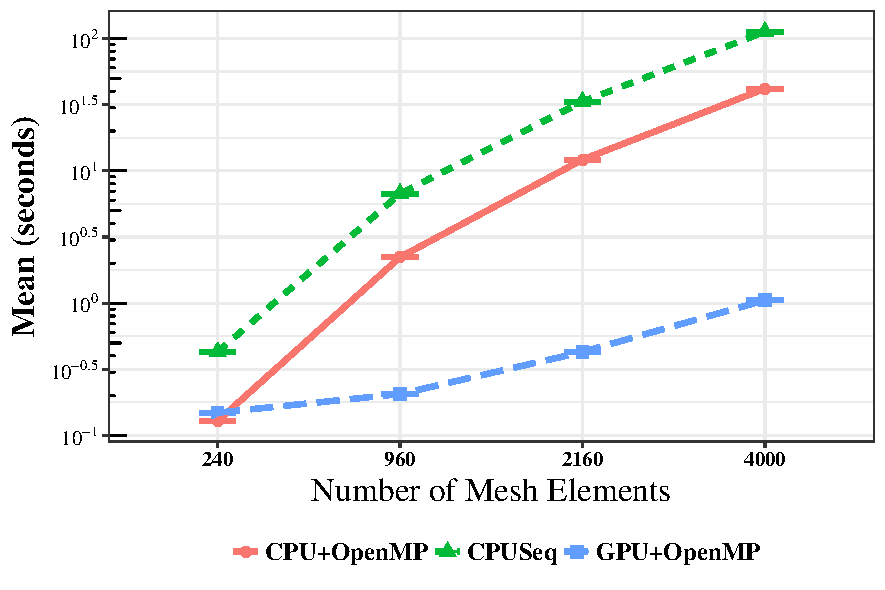
\includegraphics[scale=1.0]{results1.pdf}
\caption{Time elapsed by each implementation in logarithm scale}
\label{fig:graphic1}
\end{figure}

The speedup acquired in the $4000$ mesh elements sample with OpenMP and CUDA+OpenMP with respect to the sequential 
algorithm are $2.68$ and $106.95$ respectively. As a conclusion, the presented strategy paired with GPUs can be 
used to accelerate the overall performance of the simulation for a large number of mesh elements. This is a consequence 
of parallelizing the construction of both matrices $H$ and $G$, and the calculations in the $\texttt{Nonsingd}$ routine. 
Notice that there is a performance loss in the 260 sample between OpenMP and CUDA+OpenMP, this is caused by the high 
latency between CPU-GPU communication, thus the usage of GPUs for smaller data may not be attractive.


\section{Future Works}
The current implemented code have limitations. First, there is no logic to construct both $H$ and $G$ by blocks to create several 
GPU kernels. Second, there is also no logic to compute both $\texttt{Ghmatecd\_Nonsingd}$ and $\texttt{Ghmatecd\_Sing\_de}$ in 
parallel with respect to each other. The usage of GPUs in the singular case can also be analyzed.


%\begin{figure}[ht]
%\centering
%
\includegraphics[width=.5\textwidth]{fig1.jpg}
%\caption{A typical figure}
%\label{fig:exampleFig1}
%\end{figure}
%
%\begin{figure}[ht]
%\centering
%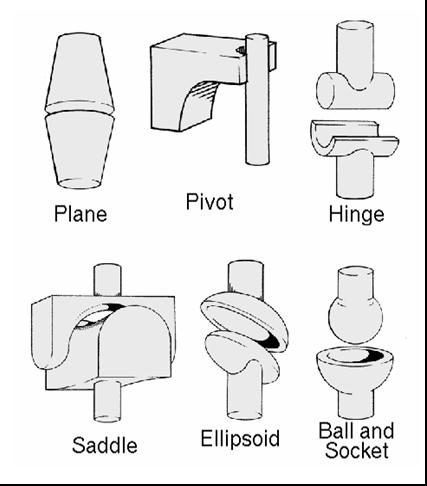
\includegraphics[width=.3\textwidth]{fig2.jpg}
%\caption{This figure is an example of a figure caption taking more than one
%  line and justified considering margins mentioned in Section~\ref{sec:figs}.}
%\label{fig:exampleFig2}
%\end{figure}


\bibliographystyle{sbc}
\bibliography{sbc-template}

\end{document}
